%%%%%%%%%%%%%%%%%%%%%%%%%%%%%%%%%%%%%%%%%
% Beamer Presentation
% LaTeX Template
% Version 1.0 (10/11/12)
%
% This template has been downloaded from:
% http://www.LaTeXTemplates.com
%
% License:
% CC BY-NC-SA 3.0 (http://creativecommons.org/licenses/by-nc-sa/3.0/)
%
%%%%%%%%%%%%%%%%%%%%%%%%%%%%%%%%%%%%%%%%%

%----------------------------------------------------------------------------------------
%	PACKAGES AND THEMES
%----------------------------------------------------------------------------------------

\documentclass[UTF8,aspectratio=169,14pt]{ctexbeamer}

\usepackage{hyperref}
\hypersetup{
	colorlinks=true,
	linkcolor=red,
	anchorcolor=blue,
	citecolor=green
}

\mode<presentation> {
	
	% The Beamer class comes with a number of default slide themes
	% which change the colors and layouts of slides. Below this is a list
	% of all the themes, uncomment each in turn to see what they look like.
	
	%\usetheme{default}
	%\usetheme{AnnArbor}
	%\usetheme{Antibes}
	%\usetheme{Bergen}
	%\usetheme{Berkeley}
	%\usetheme{Berlin}
	%\usetheme{Boadilla}
	%\usetheme{CambridgeUS}
	%\usetheme{Copenhagen}
	%\usetheme{Darmstadt}
	%\usetheme{Dresden}
	%\usetheme{Frankfurt}
	%\usetheme{Goettingen}
	%\usetheme{Hannover}
	%\usetheme{Ilmenau}
	%\usetheme{JuanLesPins}
	%\usetheme{Luebeck}
	\usetheme{Madrid}
	%\usetheme{Malmoe}
	%\usetheme{Marburg}
	%\usetheme{Montpellier}
	%\usetheme{PaloAlto}
	%\usetheme{Pittsburgh}
	%\usetheme{Rochester}
	%\usetheme{Singapore}
	%\usetheme{Szeged}
	%\usetheme{Warsaw}
	
	% As well as themes, the Beamer class has a number of color themes
	% for any slide theme. Uncomment each of these in turn to see how it
	% changes the colors of your current slide theme.
	
	%\usecolortheme{albatross}
	%\usecolortheme{beaver}
	%\usecolortheme{beetle}
	%\usecolortheme{crane}
	%\usecolortheme{dolphin}
	%\usecolortheme{dove}
	%\usecolortheme{fly}
	%\usecolortheme{lily}
	%\usecolortheme{orchid}
	%\usecolortheme{rose}
	%\usecolortheme{seagull}
	%\usecolortheme{seahorse}
	%\usecolortheme{whale}
	%\usecolortheme{wolverine}
	
	%\setbeamertemplate{footline} % To remove the footer line in all slides uncomment this line
	%\setbeamertemplate{footline}[page number] % To replace the footer line in all slides with a simple slide count uncomment this line
	
	%\setbeamertemplate{navigation symbols}{} % To remove the navigation symbols from the bottom of all slides uncomment this line
}

\usepackage{graphicx} % Allows including images
\graphicspath{{./figs/}}
\usepackage{booktabs} % Allows the use of \toprule, \midrule and \bottomrule in tables
\usepackage{longtable}
\usepackage{listings}
\usepackage{xcolor}
\lstset{numbers=left, %设置行号位置
	numberstyle=\tiny, %设置行号大小
	keywordstyle=\color{blue}, %设置关键字颜色
	commentstyle=\color[cmyk]{1,0,1,0}, %设置注释颜色
	frame=single, %设置边框格式
	escapeinside=``, %逃逸字符(1左面的键),用于显示中文
	%breaklines, %自动折行
	extendedchars=false, %解决代码跨页时,章节标题,页眉等汉字不显示的问题
	xleftmargin=2em,xrightmargin=2em, aboveskip=1em, %设置边距
	tabsize=4, %设置tab空格数
	showspaces=false %不显示空格
}
% Fonts
% \usepackage{libertine}
% \setmonofont{Courier}
\setCJKsansfont[ItalicFont=Noto Serif CJK SC Black, BoldFont=Noto Sans CJK SC Black]{Noto Sans CJK SC}

%\def\imagepath{./resources/graphics}
%\usepackage[imagepath=\imagepath]{ditaa}
%\graphicspath{ {\imagepath/} }


%\usepackage{pgfpages}
%\setbeameroption{show notes on second screen}
%%----------------------------------------------------------------------------------------
%	TITLE PAGE
%----------------------------------------------------------------------------------------

\title[第9讲]{第九讲 :进程、线程和协程} % The short title appears at the bottom of every slide, the full title is only on the title page
\subtitle{第3节:协程(coroutine)}
\author{向勇、陈渝、李国良} % Your name
\institute[清华大学] % Your institution as it will appear on the bottom of every slide, may be shorthand to save space
{
	清华大学计算机系 \\ % Your institution for the title page
	\medskip
	\textit{xyong,yuchen,liguoliang@tsinghua.edu.cn} % Your email address
}
\date{\today} % Date, can be changed to a custom date


\begin{document}

\begin{frame}
\titlepage % Print the title page as the first slide
\end{frame}

%----------------------------------------------
\begin{frame}
\frametitle{提纲} % Table of contents slide, comment this block out to remove it
\tableofcontents % Throughout your presentation, if you choose to use \section{} and \subsection{} commands, these will automatically be printed on this slide as an overview of your presentation
\end{frame}
%----------------------------------------------
%%	PRESENTATION SLIDES
%----------------------------------------------
%------------------------------------------------
\section{第3节:协程(coroutine)}% Sections can be created in order to organize your presentation into discrete blocks, all sections and subsections are automatically printed in the table of contents as an overview of the talk
% ### 9.3 协程(coroutine)
% 
\subsection{为什么引入协程}
% 
%------------------------------------------------
\begin{frame}[fragile]
    \frametitle{问题\href{https://os.phil-opp.com/async-await/\#example}{描述}}
% 
在一些并发线程数目非常多且需要频繁与外界短时交互的场景中,多线程系统的并发执行效率仍然不高。 \pause
% 

  \begin{figure}
    \centering
    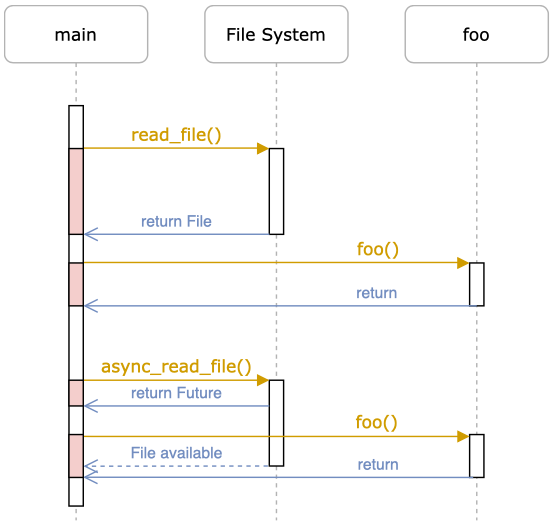
\includegraphics[width=0.45\linewidth]{figs/async-example.png}
%    \caption{async-example}
  \end{figure}



% 

\end{frame}
%------------------------------------------------
\begin{frame}[fragile]
    \frametitle{引入协程的目的}

提高线程内代码执行的并发性能和可靠性:减少线程的资源占用和切换开销,提高代码维护性; \pause
    \begin{itemize}
        \item 顺序书写异步函数代码:减弱异步函数复杂性,提高代码可读性,方便错误排查; \pause
        \item 高效支持异步函数执行:减少协程切换开销,避免线程内的并发操作冲突,提高线程内代码并发执行的性能。
    \end{itemize}
\end{frame}
% 
%------------------------------------------------
\begin{frame}
\frametitle{提纲} % Table of contents slide, comment this block out to remove it
\tableofcontents % Throughout your presentation, if you choose to use \section{} and \subsection{} commands, these will automatically be printed on this slide as an overview of your presentation
\end{frame}
%----------------------------------------------
\subsection{协程的概念}
% 
\begin{frame}[fragile]
    \frametitle{协程的概念}
% 
协程(Coroutine)是基于状态机机制实现的允许在执行过程中主动暂停和恢复的异步函数实现机制。

    \begin{itemize}
        \item \href{http://melconway.com/Home/pdf/compiler.pdf}{Design of a Separable Transition-Diagram Compiler}:1963年关于协程的论文; \pause
        \item 同步函数(ordinary function):当一个函数是同步执行时,那么当该函数被调用时不会立即返回,直到该函数所要做的事情全都做完了才返回。 \pause
        \item \href{https://www.cnblogs.com/balingybj/p/4780442.html}{异步函数}(asynchronous function):如果一个异步函数被调用时,该函数会立即返回;当该函数规定的操作任务完成时,通过回调、事件或消息机制将结果通知调用者。
    \end{itemize}

% 

\end{frame}
%------------------------------------------------
\begin{frame}[fragile]
    \frametitle{协程的模型描述}

    \begin{itemize}
        \item 状态机
            \begin{itemize}
            \item 每个状态是一个连续的代码片段执行,状态间是协程的切换; \pause
            \end{itemize}
        \item 演员模型
            \begin{itemize}
            \item 并发和合作的演员模型。每个演员有自己的任务,自愿地由调度器协调各演员的执行顺序; \pause
            \end{itemize}
        \item 生成器
        \begin{itemize}
            \item 可在指定位置暂停的执行流,由调度器遍历协调执行顺序;
        \end{itemize}
    \end{itemize}
\end{frame}
% 
%------------------------------------------------
\begin{frame}
\frametitle{提纲} % Table of contents slide, comment this block out to remove it
\tableofcontents % Throughout your presentation, if you choose to use \section{} and \subsection{} commands, these will automatically be printed on this slide as an overview of your presentation
\end{frame}
%----------------------------------------------
\subsection{协程的例子}
% 
%------------------------------------------------
\begin{frame}[fragile]
    \frametitle{Python协程示例}
% 
\href{https://en.wikipedia.org/wiki/Async/await}{Async/await}:对多种支持异步的语言中给出协程的示例程序;
% 
% 
% 
	\begin{figure}
		\centering
		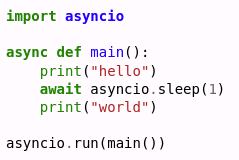
\includegraphics[width=0.5\linewidth]{figs/python-example.png}
%		\caption{python-example}
	\end{figure}


% 

\end{frame}
%------------------------------------------------
\begin{frame}[fragile]
    \frametitle{C++协程示例}
% 
	\begin{figure}
		\centering
		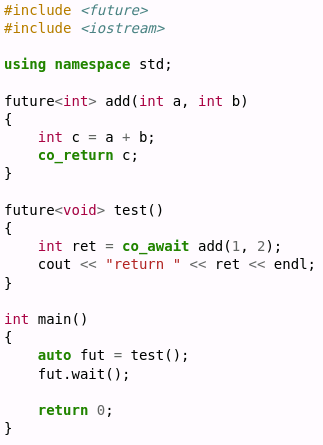
\includegraphics[width=0.35\linewidth]{figs/cpp-example.png}
		\caption{cpp-example}
	\end{figure}


% 

\end{frame}
%------------------------------------------------
\begin{frame}[fragile]
    \frametitle{Rust协程示例}
% 
	\begin{figure}
		\centering
		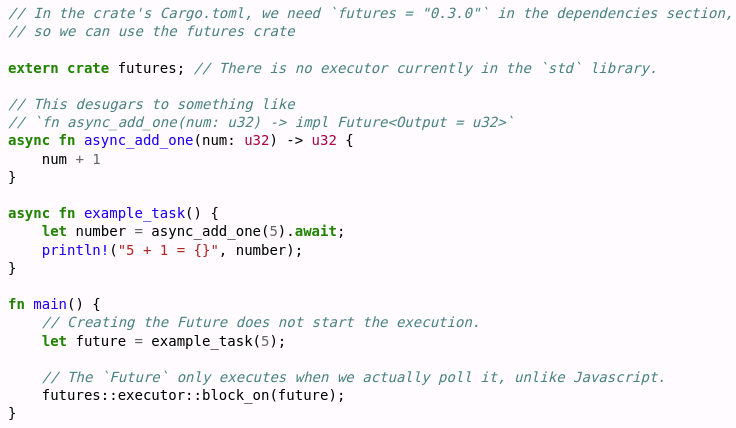
\includegraphics[width=0.8\linewidth]{figs/Rust-example.png}
%		\caption{Rust-example}
	\end{figure}

\end{frame}
% 
%------------------------------------------------
\begin{frame}
\frametitle{提纲} % Table of contents slide, comment this block out to remove it
\tableofcontents % Throughout your presentation, if you choose to use \section{} and \subsection{} commands, these will automatically be printed on this slide as an overview of your presentation
\end{frame}
%----------------------------------------------
\subsection{协程的工作原理}
% 
%------------------------------------------------
\begin{frame}[fragile]
    \frametitle{协程的工作原理}
% 
    \begin{itemize}
        \item 当协程执行中出现阻塞时,由协程调度器主动保存当前栈上数据,让权给其他可执行协程; \pause
    \begin{itemize}
        \item yield,将控制权返还给该协程的创建协程
    \end{itemize}
        \item 阻塞完后再通过协程调度器恢复栈上数据,并恢复原协程的执行。 \pause
    \begin{itemize}
        \item resume,将控制权交给一个子协程,恢复该协程的执行
    \end{itemize}

% 
    \end{itemize}
\end{frame}
%------------------------------------------------
\begin{frame}[fragile]
    \frametitle{协程的状态机\href{https://os.phil-opp.com/async-await/\#the-async-await-pattern}{描述}}
% 
	\begin{figure}
		\centering
		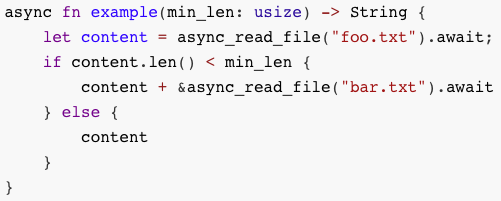
\includegraphics[width=0.5\linewidth]{figs/Rust-fsm.png}
%		\caption{Rust-fsm}
	\end{figure}

\pause
% 
	\begin{figure}
		\centering
		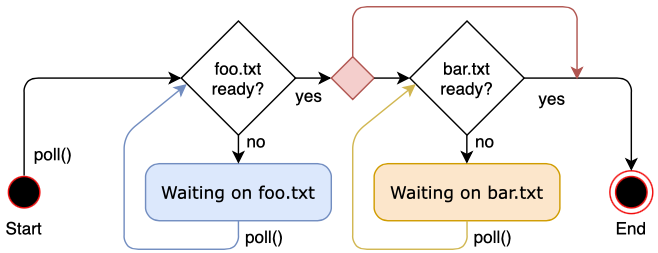
\includegraphics[width=0.6\linewidth]{figs/async-state-machine-basic.png}
%        \caption{async-state-machine-basic}
    \end{figure}


% 
% 
% 

\end{frame}
%------------------------------------------------
\begin{frame}[fragile]
    \frametitle{支持协程的线程堆栈结构}
% 
	\begin{figure}
		\centering
		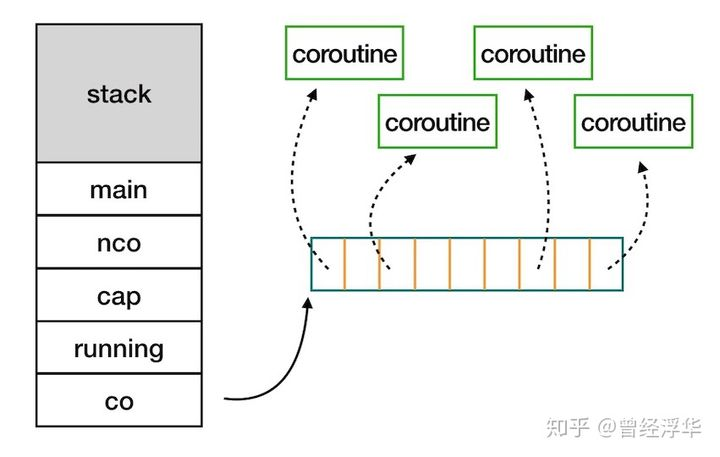
\includegraphics[width=0.75\linewidth]{figs/coroutine-memlayout.jpg}
%    \caption{coroutine-memlayout}
  \end{figure}



% 

\end{frame}
%------------------------------------------------
\begin{frame}[fragile]
    \frametitle{协程切换}
% 
	\begin{figure}
		\centering
		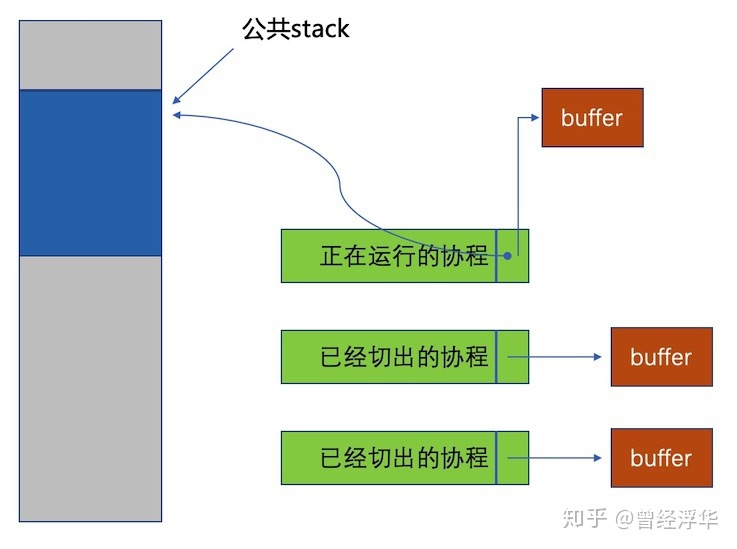
\includegraphics[width=0.4\linewidth]{figs/coroutine-stack.jpg}
%    \caption{coroutine-stack}
  \end{figure}



% 
协程运行需要栈空间,所有协程公用一块大的栈空间。当协程切出时,把自己的栈内容拷贝,当控制权再次切回时,把自己的栈内容还原到公共栈空间。

    \begin{itemize}
        \item 每个协程单独申请一块栈空间,就是用户线程。
        \item 与协程相比,用户线程的单独栈空间过小会栈溢出;太大则浪费严重。 
    \end{itemize}
\end{frame}
% 
%------------------------------------------------
\begin{frame}
\frametitle{提纲} % Table of contents slide, comment this block out to remove it
\tableofcontents % Throughout your presentation, if you choose to use \section{} and \subsection{} commands, these will automatically be printed on this slide as an overview of your presentation
\end{frame}
%----------------------------------------------
\subsection{进程、线程和协程的关系}
% 
%------------------------------------------------
\begin{frame}[fragile]
    \frametitle{\href{https://zh.wikipedia.org/wiki/\%E5\%8D\%8F\%E7\%A8\%8B}{协程与函数}}

    \begin{itemize}
        \item 函数
    \begin{itemize}
        \item 函数可以调用其他函数,调用函数等待被调用函数结束后继续执行
        \item 函数的入口点是唯一的,函数被调用时是从入口点开始执行
        \item 函数在结束时一次性返回全部结果
    \end{itemize}
    \end{itemize}
    \begin{itemize}
        \item 协程
    \begin{itemize}
        \item 协程可以调用其他协程,但调用协程在等待被调用协 程结束前可以执行其他协程
        \item 协程可有多个入口点,协程被调用时是第一个入口点开始执行,每个暂停返回出口点都是再次被调用执行时的入口点
        \item 协程在暂停返回时可返回部分结果
    \end{itemize}
    \end{itemize}

% 

\end{frame}
%------------------------------------------------
\begin{frame}[fragile]
    \frametitle{\href{https://www.cnblogs.com/theRhyme/p/14061698.html}{协程与线程}}

    \begin{itemize}
        \item 协程的开销远远小于线程的开销:不需要独立的栈空间;切换时需要保存和恢复的数据少; \pause
        \item 在多核处理器的环境下, 多个线程是可并行的;协程是并发的,任何时刻同一线程内只有一个协程在执行,其他协程处于暂停状态; \pause
        \item 线程切换可以是抢先式或非抢先式;而同线程内的协程切换只有非抢先式;
    \end{itemize}

% 

\end{frame}
%------------------------------------------------
\begin{frame}[fragile]
    \frametitle{进程、线程和协程\href{https://www.cnblogs.com/theRhyme/p/14061698.html}{比较}}
% 
	\begin{figure}
		\centering
		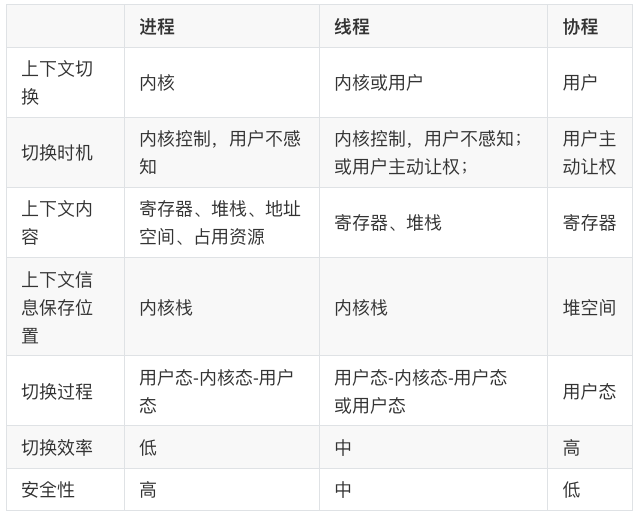
\includegraphics[width=0.55\linewidth]{figs/proc-thread-coroutine.png}
%		\caption{proc-thread-coroutine}
	\end{figure}
\end{frame}
%------------------------------------------------
\end{document}
